\section{Finite-regime definition of entanglement-dynamic topology}

We define Entanglement-Dynamic Topology (EDT) as a \emph{finite parameter window} in which a system supports simultaneously structured, compatible, and dynamically useful quantum-resource behavior. The relevant control coordinate is denoted generically by $x$, where $x$ may represent momentum $k$, a phonon normal-mode coordinate $Q$, loop or interaction strength $\lambda$, circuit depth, pulse number $N$, pulse spacing $\tau$, or another experimentally accessible control variable. In this sense, EDT is not tied to a single platform-specific parameterization; it is a regime criterion applied to whichever coordinate organizes the competition between structure generation and resource degradation.

The EDT regime is defined as the set
\begin{equation}
\Delta_{\rm EDT}
=
\{x: S_{\rm pair}(x) > S_{\rm pair}^{(0)},
R_{\rm quad}(x) < R_{\rm quad}^{(0)},
S_{\rm dyn}(x) > S_{\rm dyn}^{(0)} \},
\end{equation}
where each inequality expresses a measurable or computable condition for finite-regime viability.

The first term, $S_{\rm pair}(x)$, is a curvature-pairing or branch-compatibility score. In materials examples, it quantifies how well paired curvature branches remain mutually compatible within a local description near a degeneracy or avoided crossing. In dynamical settings, it can be interpreted more generally as a compatibility measure between the relevant structured branches or channels supporting the candidate regime. The reference value $S_{\rm pair}^{(0)}$ sets the minimum compatibility required for the regime to be considered organized rather than accidental.

The second term, $R_{\rm quad}(x)$, is the residual error of a local quadratic model. It measures how well the relevant structure can be approximated by a stable local expansion around the candidate operating point. In the K$_3$C$_{60}$ analysis, this is the residual associated with paired quadratic fits to curvature branches. The threshold $R_{\rm quad}^{(0)}$ therefore separates regions where the local model remains coherent from regions where the structure becomes too irregular, too sharp, or too weakly organized to support a finite EDT window.

The third term, $S_{\rm dyn}(x)$, is a dynamical resource score. Its exact form depends on the platform. In the plaquette model, it is built from operator spreading and long-time correlation retention. In sensing problems, it may be a filtered response or sensitivity proxy combining signal accumulation with coherence and control fidelity. In all cases, $S_{\rm dyn}(x)$ is intended to capture whether the candidate region is not only geometrically structured but also dynamically useful. The threshold $S_{\rm dyn}^{(0)}$ enforces that the regime remain operationally relevant rather than merely geometrically identifiable.

When robustness information is available, we also introduce an optional score $S_{\rm robust}(x)$ measuring stability under threshold changes, parameter perturbations, or approximate implementation such as Trotterization. This quantity is not required to identify an EDT window at the most basic level, but it is useful for ranking candidate regimes by their resilience to modeling choices and control imperfections.

To summarize these ingredients in a single bounded diagnostic, we define a composite normalized score
\begin{equation}
S_{\rm EDT}(x) = S_{\rm pair}(x)\,S_{\rm quad}(x)\,S_{\rm dyn}(x)\,S_{\rm robust}(x),
\end{equation}
with
\begin{equation}
S_{\rm quad}(x) = \exp[-R_{\rm quad}(x)/R_0],
\end{equation}
where $R_0$ sets the residual scale. This choice ensures that improved local quadratic consistency increases the score monotonically while large residuals suppress it smoothly rather than through a discontinuous rule. When an explicit robustness measure is not available, one may set $S_{\rm robust}(x)=1$ and retain the three-factor finite-regime diagnostic.

Within this formulation, EDT is identified not by the maximization of any single quantity, but by the existence of an \emph{interior region} in control space where branch compatibility remains high, local structure remains well described, and dynamical usefulness remains above threshold. The resulting window is finite by construction: outside it, at least one of the conditions defining $\Delta_{\rm EDT}$ fails.

\paragraph*{Clarification.}

EDT is not a new microscopic interaction and not a new quantum resource type. It is a finite-regime organization principle identifying where existing quantum resources are simultaneously generated, structured, and dynamically stable.

\subsection{Physical Origin and Organization}

Within the present manuscript, the microscopic origin of the finite-regime structure is non-adiabatic coupling between electronic and lattice degrees of freedom~\cite{Mead1979,Yarkony1996,Giustino2017}. Near degeneracies and band crossings, the second-order response of electronic energies to normal-mode coordinates generates curvature fields that organize the local structure of the coupled manifold. These curvature fields provide the main materials-side diagnostic used below in K$_3$C$_{60}$, where the finite EDT window is extracted through paired curvature fits and residual thresholding.

The same finite-regime logic extends naturally beyond momentum-space diagnostics. In the plaquette model, the control coordinate is the loop strength $\lambda$, and the relevant dynamical score is built from operator spreading and long-time correlation persistence. In the NV XY8 case study, the control coordinates are pulse number $N$ and pulse spacing $\tau$, and the dynamical score is replaced by a sensing-oriented resource proxy combining filter response, coherence, pulse fidelity, and duty-cycle overhead. These examples differ in physical realization, but they share the same finite-window definition.

\begin{figure*}[t]
\centering
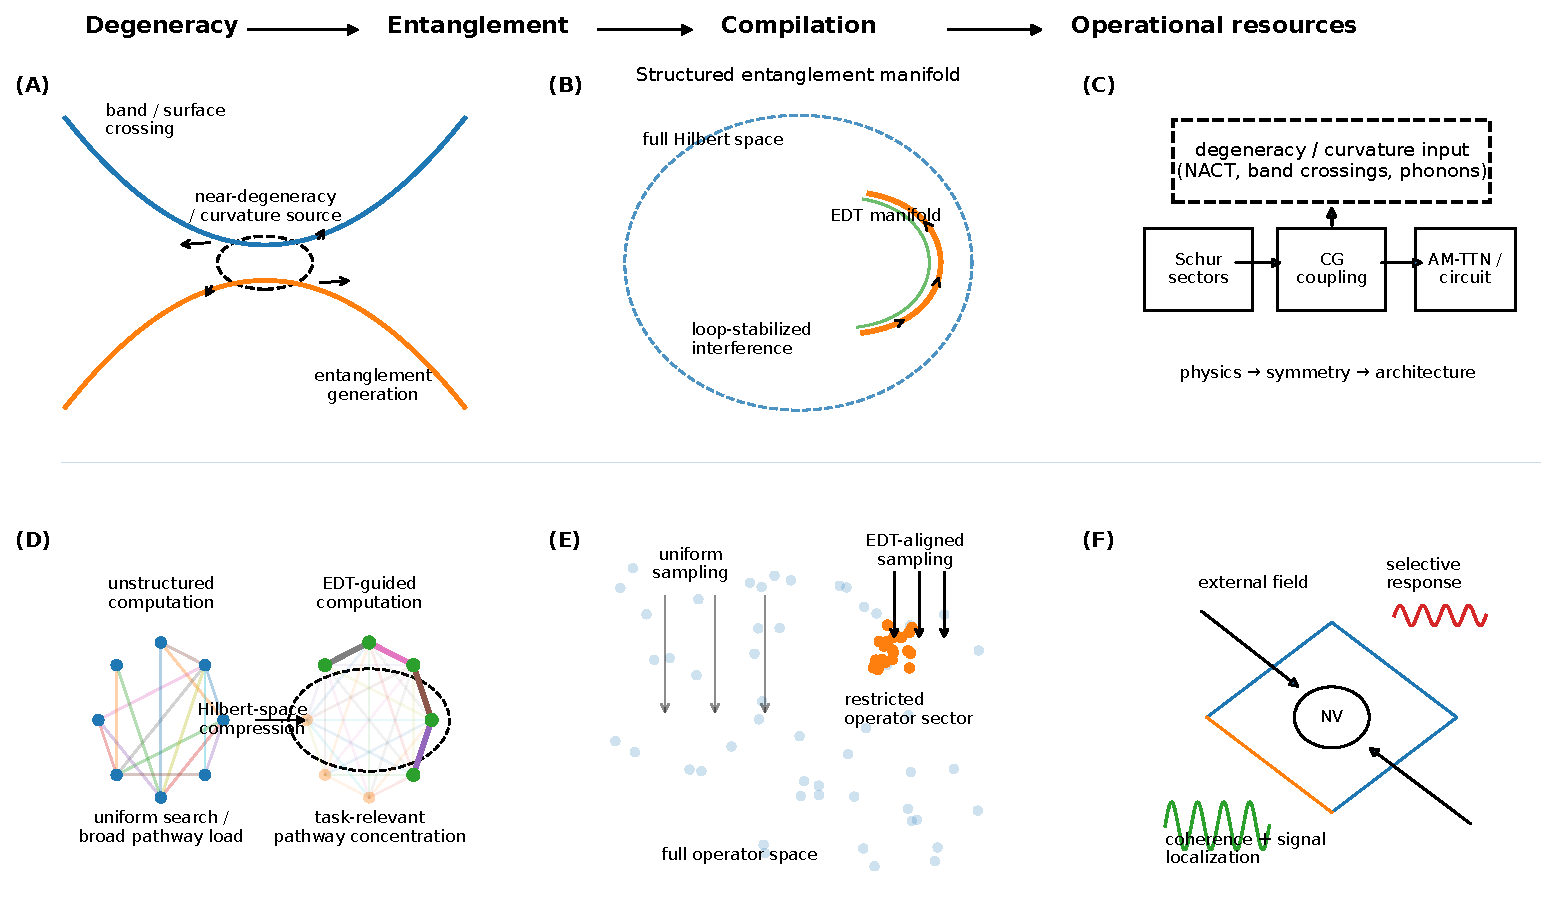
\includegraphics[width=0.95\linewidth]{fig1_edt_framework_camera_ready.pdf}
\caption{\textbf{Physical origin and organization of EDT.}
(A) Near degeneracies and band crossings act as curvature sources, where non-adiabatic coupling generates entanglement.
(B) A structured entanglement manifold is embedded within the full Hilbert space and stabilized by loop-induced interference.
(C) Physical structure can be compiled into symmetry-adapted architectures, including Schur sectors, Clebsch-Gordan coupling, and circuit representations.
(D) EDT-guided evolution concentrates dynamics into structured pathways rather than unstructured Hilbert-space exploration.
(E) Task-relevant operator sectors can be selectively sampled under EDT alignment.
(F) In sensing platforms, structured manifolds enable selective response and coherence localization.}
\label{fig:edt_concept}
\end{figure*}

\paragraph*{From non-adiabatic coupling to an effective EDT Hamiltonian.}

Starting from the electron--phonon Hamiltonian
\begin{equation}
H = H_e(\mathbf{r};\{Q_\alpha\}) + \sum_\alpha \left(\frac{P_\alpha^2}{2M_\alpha} + \frac{1}{2} M_\alpha \omega_\alpha^2 Q_\alpha^2\right),
\end{equation}
non-adiabatic effects arise from the dependence of the electronic Hamiltonian on normal-mode coordinates $Q_\alpha$~\cite{BornOppenheimer1927,Mead1979,Yarkony1996}. Expanding $H_e$ to second order,
\begin{equation}
H_e(\{Q_\alpha\}) \approx H_e^{(0)} + \sum_\alpha Q_\alpha \,\partial_\alpha H_e + \frac{1}{2}\sum_{\alpha\beta} Q_\alpha Q_\beta \,\partial_\alpha \partial_\beta H_e,
\end{equation}
and projecting onto an adiabatic electronic basis $\{|n\rangle\}$ yields NACT matrix elements
\begin{equation}
A^{(\alpha)}_{mn} = \langle m | \partial_{Q_\alpha} | n \rangle,
\end{equation}
which generate off-diagonal mixing and geometric phases~\cite{Berry1984}. Eliminating fast phonon coordinates produces an effective electronic Hamiltonian with curvature-mediated interactions~\cite{SchriefferWolff1966,LangFirsov1962},
\begin{equation}
H_{\mathrm{eff}} \simeq H_0 + \sum_{\langle i,j\rangle} J_{ij}\, Z_i Z_j + \sum_p \lambda_p\, W_p,
\end{equation}
where $J_{ij}$ arises from second-order curvature processes and $W_p$ denotes loop operators generated by multi-mode interference of NACT fields.

At the operational level, these structures define a computational framework. The structured manifold can be compiled into symmetry-adapted architectures, including Schur-sector decompositions, Clebsch--Gordan coupling trees, and tensor-network representations, enabling Hilbert-space compression and concentration of dynamics along task-relevant pathways~\cite{Bacon2006}. In this way, the finite-regime definition of EDT connects microscopic curvature diagnostics to dynamical models and platform-level control studies within a single quantitative language.
